%%%%%%%%%%%%%%%%%%%%%%%%%%%%%%%%%%%%%%%%%%%%%%%%%%%%%%%%%%%%%%%%%%%%%%%%%%
% Layer stacks of the planar transformer (Exercise 07, Task 3)
%%%%%%%%%%%%%%%%%%%%%%%%%%%%%%%%%%%%%%%%%%%%%%%%%%%%%%%%%%%%%%%%%%%%%%%%%%

\begin{figure}[htb]
	\begin{center}
		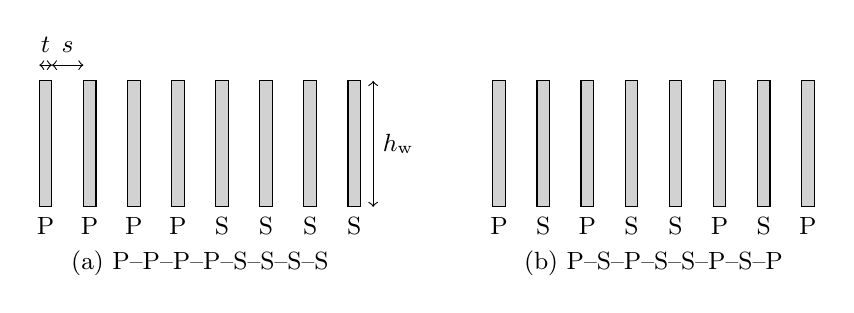
\begin{tikzpicture}[scale=0.8, every node/.style={font=\small}]
			% (a) PPPP-SSSS
			\foreach \k/\l in {0/P,1/P,2/P,3/P,4/S,5/S,6/S,7/S}{
					\fill[gray!35] (0.7*\k,0) rectangle (0.7*\k+0.2,2.0);
					\draw (0.7*\k,0) rectangle (0.7*\k+0.2,2.0);
					\node at (0.7*\k+0.1,-0.3) {\l};
				}
			\node at (2.55,-0.9) {(a) P--P--P--P--S--S--S--S};
			% dimensions
			\draw[<->] (0,2.25) -- (0.2,2.25);
			\node[anchor=south] at (0.1,2.3) {$t$};
			\draw[<->] (0.2,2.25) -- (0.7,2.25);
			\node[anchor=south] at (0.45,2.3) {$s$};
			\draw[<->] (5.3,0) -- (5.3,2.0) node[midway, right]{$h_\mathrm{w}$};
			% (b) PSPSSPSP
			\begin{scope}[xshift=7.2cm]
				\foreach \k/\l in {0/P,1/S,2/P,3/S,4/S,5/P,6/S,7/P}{
						\fill[gray!35] (0.7*\k,0) rectangle (0.7*\k+0.2,2.0);
						\draw (0.7*\k,0) rectangle (0.7*\k+0.2,2.0);
						\node at (0.7*\k+0.1,-0.3) {\l};
					}
				\node at (2.55,-0.9) {(b) P--S--P--S--S--P--S--P};
			\end{scope}
		\end{tikzpicture}
	\end{center}
	\caption{Cross-section of the two layer stacks (copper layers of thickness $t$, insulation $s$, winding breadth $h_\mathrm{w}$; not to scale)}
	\label{fig:ex07_stack}
\end{figure}
